\chapter{Preparing Data for Models}

Here is a mystery penguin: bill 40.3 mm long and 18.5 mm deep, flipper 196 mm, mass 4,350 g. Which penguin in
the data set is most like it? A natural idea is to treat each penguin as a point with four coordinates and find
the closest point, the way you would find the distance between two points on a graph:
$$d = \sqrt{(\Delta \text{bill length})^2 + (\Delta \text{bill depth})^2 + (\Delta \text{flipper})^2 +
(\Delta \text{mass})^2}$$

Try it, and the answer is a Gentoo with exactly the same mass, even though its bill is 5 mm shallower and its
flipper 12 mm longer. Meanwhile, an Adelie that matches the mystery penguin almost perfectly (41.5, 18.3, 195,
4,300) is ``farther away,'' because its mass differs by 50. Fifty \emph{grams} is nothing for a penguin, but
the formula cannot tell grams from millimeters; it just sees the number 50.

Real data needs preparing before most models can use it. This chapter covers the two most common jobs:
putting numbers on comparable scales, and turning categories into numbers.

\section{Why Scale Matters}
Each feature adds its squared difference to the distance. Figure~\ref{fig:distance-shares} shows how much of the
squared distance between the mystery penguin and that near-twin Adelie comes from each measurement.

\begin{figure}[H]
\centering
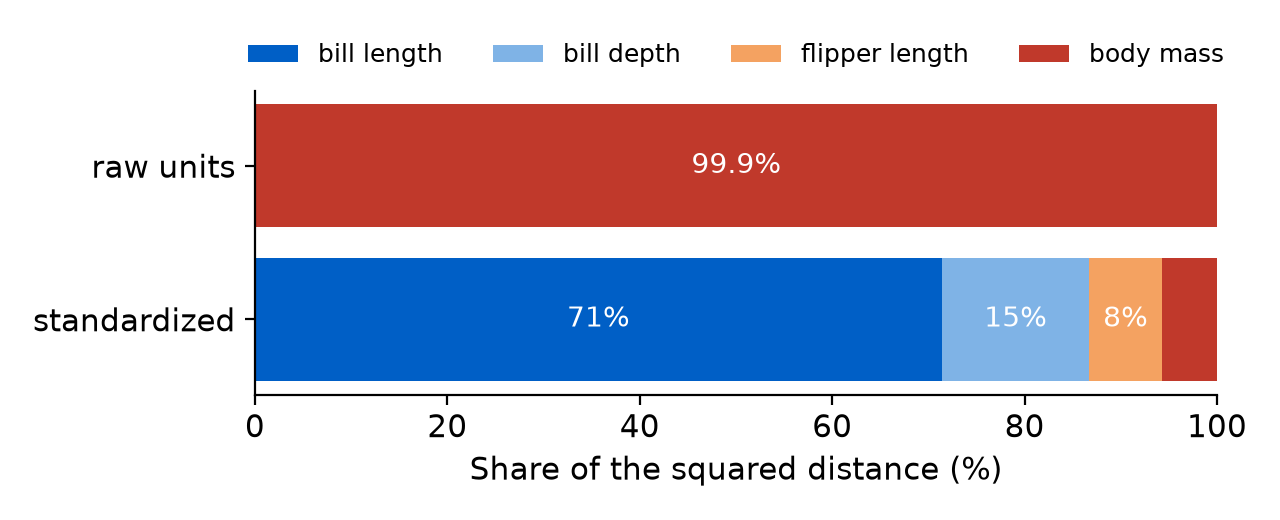
\includegraphics[width=0.85\textwidth]{distance_shares.png}
\caption{Where the distance comes from. In raw units, body mass accounts for 99.9\% of it, because masses are
measured in thousands. After standardizing, all four measurements contribute.}
\label{fig:distance-shares}
\end{figure}

In raw units, the bills and flippers might as well not exist. This matters for any method that combines
features by adding them up: nearest neighbors, clustering, gradient descent, and neural networks.

Here is the experiment, in \filename{nearest.py}:

\begin{minted}{python}
import numpy as np
from penguins import load_penguins

data = load_penguins()
names = ["bill_length_mm", "bill_depth_mm", "flipper_length_mm", "body_mass_g"]
X = np.column_stack([data[name] for name in names])   # 333 rows, 4 columns
species = data["species"]

def nearest(features, i):
    """Row number of the penguin closest to penguin i."""
    distances = np.sqrt(np.sum((features - features[i])**2, axis=1))
    distances[i] = np.inf          # do not count the penguin itself
    return np.argmin(distances)

mystery = 91
print("Mystery penguin:", species[mystery], X[mystery])

j = nearest(X, mystery)
print("Nearest in raw units:", species[j], X[j])

Z = (X - X.mean(axis=0)) / X.std(axis=0)   # standardize every column
j = nearest(Z, mystery)
print("Nearest after standardizing:", species[j], X[j])
\end{minted}

\begin{verbatim}
Mystery penguin: Adelie [  40.3   18.5  196.  4350. ]
Nearest in raw units: Gentoo [  44.    13.6  208.  4350. ]
Nearest after standardizing: Adelie [  41.5   18.3  195.  4300. ]
\end{verbatim}

\verb|np.column_stack| puts the four arrays side by side as columns. In \verb|features - features[i]|, NumPy
subtracts one penguin's row from every row at once (this is called \newterm{broadcasting}\index{broadcasting}),
and \verb|axis=1| sums across each row. The line that makes \verb|Z| is the subject of the next section.

This is not a lucky example. If you label every penguin with the species of its nearest neighbor, you are right
86.8\% of the time in raw units and 98.2\% of the time after standardizing.

\section{Standardization}\index{standardization}
\newterm{Standardization} rescales a feature so its mean is 0 and its standard deviation is 1. For a feature
with mean $\mu$ and standard deviation $\sigma$,
$$z = \frac{x - \mu}{\sigma}$$
Each standardized value says how many standard deviations the original value is above or below the mean. It is
the same $z$-score as in the Shape, Position, and Outliers chapter.

\textbf{Example}: Standardize the values $2, 4, 6, 8$.

\textbf{Solution}: The mean is $\mu = 5$. Using the population standard deviation (dividing by $n$, as NumPy's
\verb|std| does), $\sigma = \sqrt{\frac{9 + 1 + 1 + 9}{4}} = \sqrt{5} \approx 2.236$. So
$$\frac{2 - 5}{2.236} \approx -1.342, \quad \frac{4 - 5}{2.236} \approx -0.447, \quad
\frac{6 - 5}{2.236} \approx 0.447, \quad \frac{8 - 5}{2.236} \approx 1.342$$

Standardization changes the axis, not the shape (Figure~\ref{fig:standardized-hist}). Skewed data stays skewed,
and outliers stay outliers.

\begin{figure}[H]
\centering
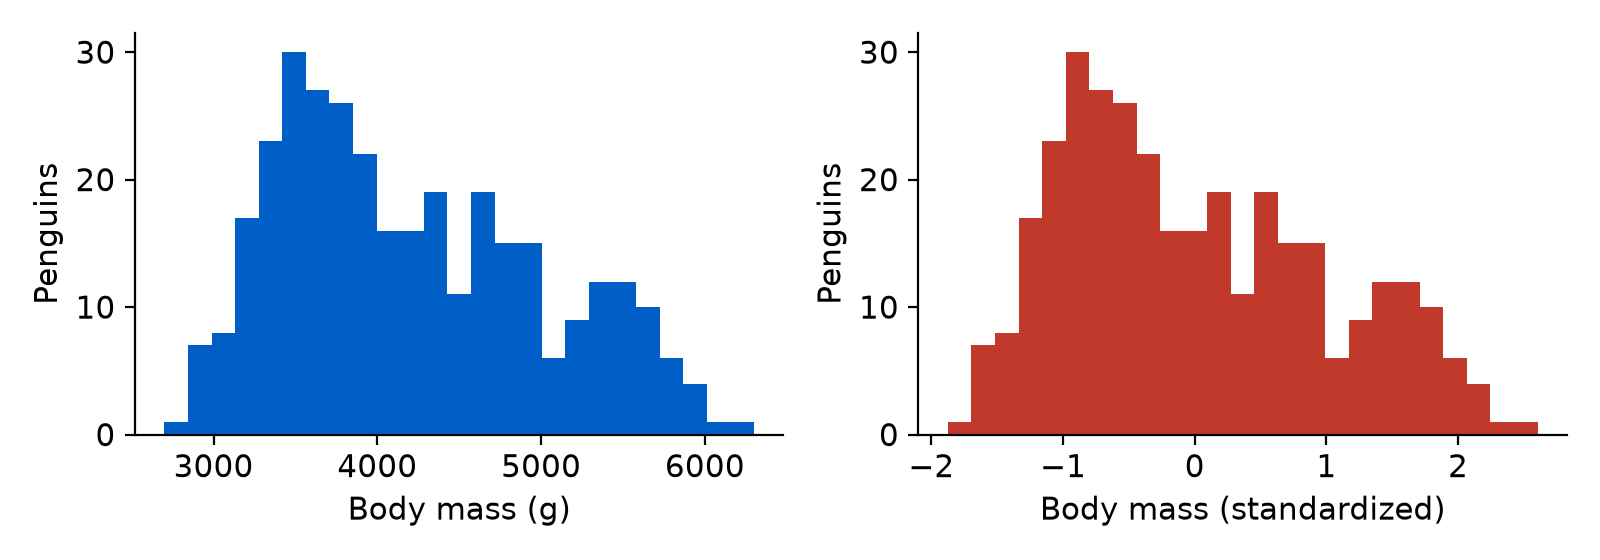
\includegraphics[width=0.85\textwidth]{standardized_hist.png}
\caption{Penguin body masses before and after standardizing. The histograms are identical except for the
numbers on the horizontal axis.}
\label{fig:standardized-hist}
\end{figure}

Another option, \newterm{min-max scaling}\index{min-max scaling}, squeezes each feature into the range 0 to 1:
$$x' = \frac{x - \min}{\max - \min}$$
It is common for things that are naturally bounded, like pixel brightness. Standardization is the usual default,
because a single extreme value can squash all the others into a tiny corner of $[0, 1]$.

\subsection{Which Methods Need It?}
\begin{center}
\begin{tabular}{l l >{\raggedright\arraybackslash}p{5.2cm}}
\textbf{Method} & \textbf{Needs scaling?} & \textbf{Why} \\
\hline
Least squares regression & no & gives the same predictions either way; scaling only makes coefficients easier to compare \\
Gradient descent & yes & unscaled features make it crawl \\
$k$-nearest neighbors, $k$-means & yes & they are built on distances \\
Naive Bayes & no & it treats each feature separately \\
Decision trees and forests & no & a split like ``mass $< 4000$'' works the same in any units \\
Neural networks & yes & training is slow and unstable without it \\
\end{tabular}
\end{center}

\section{Categories Become Numbers}\index{categorical variable}
Species, island, and sex are \newterm{categorical variables}: their values are labels, not numbers. Most models
need numbers. Why not just number the islands, Biscoe $= 1$, Dream $= 2$, Torgersen $= 3$? Because then a model
would believe that Torgersen is ``bigger'' than Biscoe, and that Dream sits exactly halfway between them. The
islands have no such order.

\newterm{One-hot encoding}\index{one-hot encoding} gives each category its own column, which is 1 when the row
has that category and 0 otherwise:

\begin{center}
\begin{tabular}{c|ccc}
Island & \texttt{is\_Biscoe} & \texttt{is\_Dream} & \texttt{is\_Torgersen} \\
\hline
Torgersen & 0 & 0 & 1 \\
Biscoe & 1 & 0 & 0 \\
Dream & 0 & 1 & 0 \\
Biscoe & 1 & 0 & 0 \\
\end{tabular}
\end{center}

Every row has exactly one 1. A feature with two categories, such as sex, needs only a single 0-or-1 column.

\subsection{The Dummy Variable Trap}\index{dummy variable trap}
One of those three columns is redundant. If you know \texttt{is\_Dream} and \texttt{is\_Torgersen}, you know
\texttt{is\_Biscoe}: it is $1 - \texttt{is\_Dream} - \texttt{is\_Torgersen}$. In a linear regression, which
already has an intercept, the three columns add up to the column of 1s that the intercept multiplies, so the
regression cannot tell their effects apart. The fix is to drop one column. The dropped category becomes the
\newterm{baseline}\index{baseline category}, and each remaining coefficient measures the difference from it.
Trees and neural networks do not mind the extra column.

For categories that \emph{do} have an order, like small, medium, and large, or freshman through senior, a
single column of numbers (1, 2, 3, 4) that respects the order is often better.

\section{Missing Values}\index{missing values}
Eleven of the 344 penguins are missing a measurement, so \pyfunction{load\_penguins} quietly drops them. With
so few, that is fine. With more, you would lose too much data, and the usual fix is to \emph{fill in}, or
\newterm{impute}\index{imputation}, each missing value with the training set's mean (for numbers) or most
common value (for categories). Sometimes you also add a 0-or-1 column recording that the value was missing,
since being missing can itself carry information.

\section{Putting It Together}
Here is a full feature matrix for the penguins: four standardized measurements, two island columns, and a sex
column. Note that the mean and standard deviation come from the training rows only, so no information leaks from
the test set. Create \filename{prepare.py}:

\begin{minted}{python}
import numpy as np
from penguins import load_penguins

data = load_penguins()
n = len(data["species"])
order = np.random.default_rng(seed=1).permutation(n)
train, test = order[:250], order[250:]

# 1. Numbers: standardize with the TRAINING mean and standard deviation
names = ["bill_length_mm", "bill_depth_mm", "flipper_length_mm", "body_mass_g"]
numbers = np.column_stack([data[name] for name in names])
mean = numbers[train].mean(axis=0)
sd = numbers[train].std(axis=0)
scaled = (numbers - mean) / sd

# 2. Categories: one-hot encode the island, dropping one column (Biscoe)
islands = np.array(["Dream", "Torgersen"])
island_columns = (data["island"][:, None] == islands[None, :]).astype(float)

# 3. Two categories need only one column
male = (data["sex"] == "male").astype(float)[:, None]

X = np.hstack([scaled, island_columns, male])
print("Feature matrix:", X.shape)
print("First penguin: ", np.round(X[0], 2))
# Adding 0.0 turns a printed -0.0 into 0.0
print("Training means:", np.round(X[train, :4].mean(axis=0), 2) + 0.0)
print("Test means:    ", np.round(X[test, :4].mean(axis=0), 2) + 0.0)
\end{minted}

\begin{verbatim}
Feature matrix: (333, 7)
First penguin:  [-0.9   0.76 -1.46 -0.62  0.    1.    1.  ]
Training means: [0. 0. 0. 0.]
Test means:     [-0.02  0.   -0.11 -0.24]
\end{verbatim}

The one-hot line uses broadcasting again. \verb|data["island"][:, None]| is a column of 333 islands, and
\verb|islands[None, :]| is a row of two; comparing them gives a $333 \times 2$ table of \verb|True| and
\verb|False|, and \verb|astype(float)| turns those into 1s and 0s.

The first penguin, from Torgersen, gets $(0, 1)$ in the island columns, and its last 1 says it is male. The
training means are exactly 0, as they must be. The test means are close to 0 but not equal to it, and that is
correct: the test penguins were scaled with the training statistics, as if they had arrived later.

\begin{Exercise}[label=std1, title=Standardize a value]
A feature has mean 50 and standard deviation 10. What is the standardized value of 65?
\end{Exercise}
\begin{Answer}[ref=std1]
$z = \frac{65 - 50}{10} = 1.5$.
\end{Answer}

\begin{Exercise}[label=std3, title=Which test went better?]
You scored 85 on a math test (class mean 75, standard deviation 5) and 90 on a science test (class mean 85,
standard deviation 10). Relative to your class, which test went better?
\end{Exercise}
\begin{Answer}[ref=std3]
Math: $z = \frac{85 - 75}{5} = 2$. Science: $z = \frac{90 - 85}{10} = 0.5$. Your math score is two standard
deviations above the mean, and your science score only half a standard deviation above. Math went better, even
though the raw score was lower.
\end{Answer}

\begin{Exercise}[label=std2, title=Leakage]
A student computes $\mu$ and $\sigma$ from all the data, then splits it into training and test sets. What is
the problem?
\end{Exercise}
\begin{Answer}[ref=std2]
The test data helped determine the scaling, so information from the test set has leaked into training. Compute
$\mu$ and $\sigma$ from the training set only, and apply those same values to the test set.
\end{Answer}

\begin{Exercise}[label=oh1, title=Encode a variable]
Write the one-hot encoding of the pets cat, dog, fish, cat, using three columns in that order.
\end{Exercise}
\begin{Answer}[ref=oh1]
$(1,0,0)$, $(0,1,0)$, $(0,0,1)$, $(1,0,0)$.
\end{Answer}

\begin{Exercise}[label=oh2, title=Dropping a column]
A regression uses the island variable encoded as three columns. Why should one column be dropped?
\end{Exercise}
\begin{Answer}[ref=oh2]
The three columns add up to 1 in every row, which is the same as the intercept's column of 1s. The regression
cannot separate their effects, so its coefficients are not determined. Dropping one column fixes this, and the
dropped island becomes the baseline.
\end{Answer}

\begin{Exercise}[label=std4, title={Min-max scaling}]
Add min-max scaling to \filename{nearest.py} and find the mystery penguin's nearest neighbor with it. What
values does penguin 0 (bill 39.1 mm long and 18.7 mm deep, flipper 181 mm, mass 3,750 g) get after min-max
scaling?
\end{Exercise}
\begin{Answer}[ref=std4]
\begin{minted}{python}
M = (X - X.min(axis=0)) / (X.max(axis=0) - X.min(axis=0))
j = nearest(M, mystery)
print("Nearest after min-max scaling:", species[j], X[j])
print(np.round(M[0], 3))
\end{minted}
The nearest neighbor is the same near-twin Adelie (41.5, 18.3, 195, 4300). Penguin 0 becomes
$(0.255, 0.667, 0.153, 0.292)$: for example, its bill length of 39.1 mm is 25.5\% of the way from the shortest
bill (32.1 mm) to the longest (59.6 mm).
\end{Answer}

\begin{Exercise}[label=oh3, title={One-hot species}]
Write one line of NumPy that one-hot encodes the species into three columns, and check that every row adds up
to 1.
\end{Exercise}
\begin{Answer}[ref=oh3]
\begin{minted}{python}
kinds = np.unique(data["species"])          # Adelie, Chinstrap, Gentoo
onehot = (data["species"][:, None] == kinds[None, :]).astype(float)
print(onehot.shape, np.all(onehot.sum(axis=1) == 1))
\end{minted}
It prints \verb|(333, 3) True|.
\end{Answer}
